\pgfmathdeclarefunction{ImpedanzBetrag}{3}{%
  \pgfmathparse{#1/sqrt(1+(x*#2-1/(x*#3))^2*#1^2)}%
}
\pgfmathdeclarefunction{ImpedanzStromL}{3}{%
	\pgfmathparse{#1}%
}
	%\pgfmathparse{R/sqrt(1+(xC-1/xL)^2*R^2)}
	%R=1000
	%C=1*10^(-6)=0.000001
	%L=10*10^-(3)=0.01

\makebox{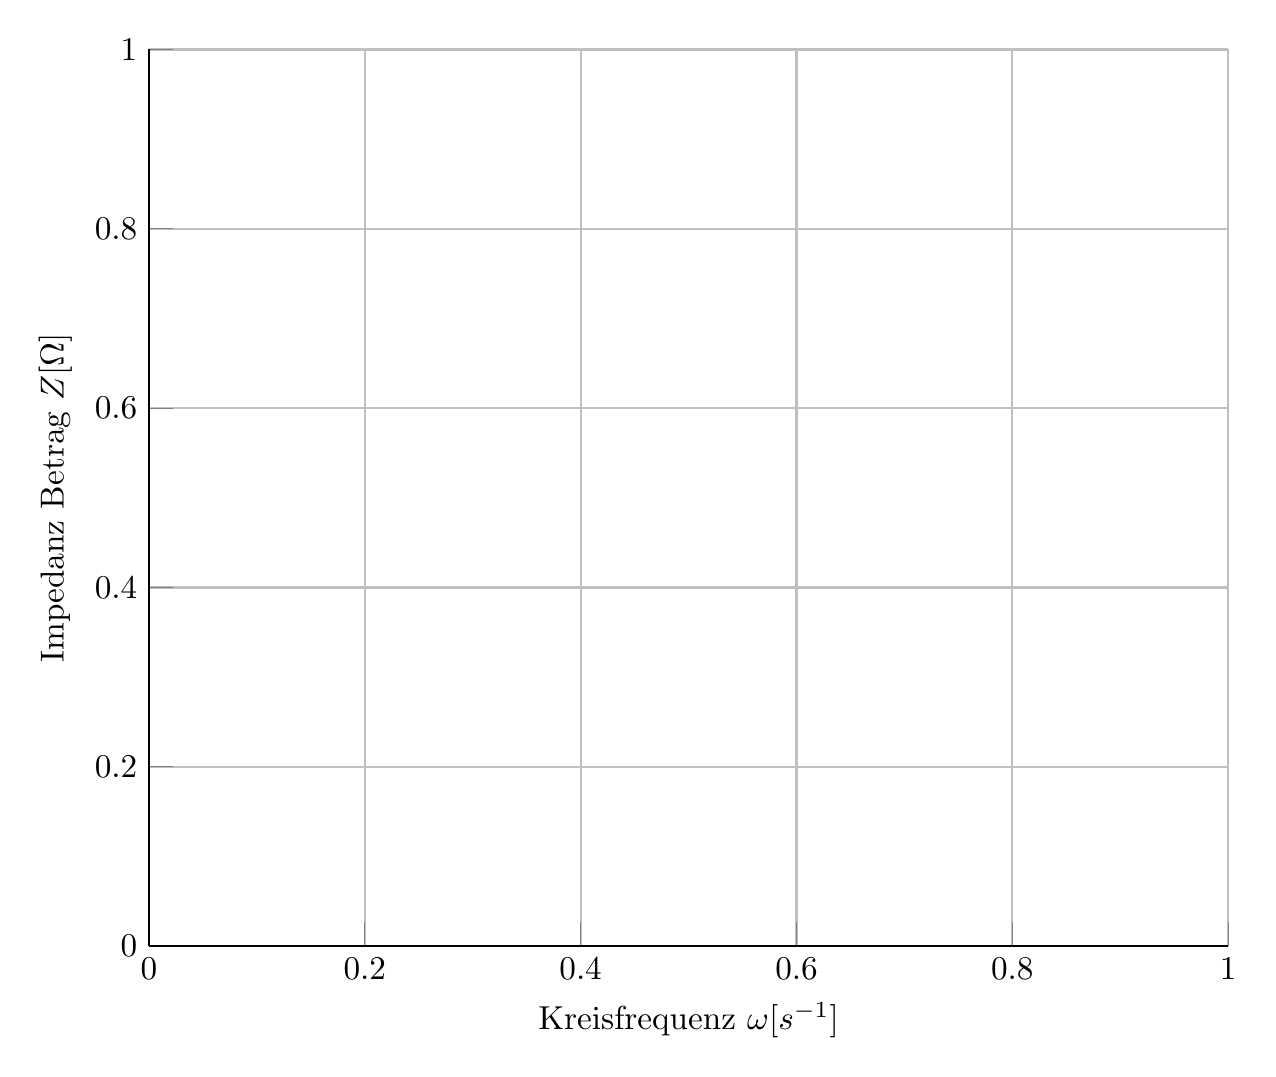
\begin{tikzpicture}[scale=2, every node/.style={scale=0.6}]
\begin{axis}[
  no markers,
  domain=5*10^3:15*10^3,
  %hide x axis=true,
  %hide y axis=true,
  samples=500,
  %line width = 1.5pt,
  axis x line*=bottom,
  axis y line*=left,
  xtick={4000,5000,...,15000,16000},
  ytick={0,100,200,...,1000},
  ymin=0,
  xmin=4000,
  xmax=16000,
  enlargelimits=false,
  clip=false,
  axis on top,
  grid = major,
  xlabel={Kreisfrequenz $\omega[s^{-1}]$},
  ylabel={Impedanz Betrag $Z[\Omega]$}
  ]
  %\addplot{ImpedanzBetrag(1000, 0.000001, 0.01)};
%   \addplot[dashed] plot coordinates  {
%   	(9000,707)
%   	(16000,707)
%   };
%   
%   \addplot[dashed] plot coordinates  {
%   	(9500,780)
%   	(9500,0)
%   };
%   \addplot[dashed] plot coordinates  {
%   	(10500,780)
%   	(10500,0)
%   };
%   \node[coordinate,label=right:{$1/\sqrt{2}$}]
%     at (axis cs:16000,707) {};
%   \node[coordinate,label=below:{$\omega_1$}]
%     at (axis cs:9500,-30) {};
%   \node[coordinate,label=below:{$\omega_2$}]
%     at (axis cs:10500,-30) {};
\end{axis}
\end{tikzpicture}}


